% Created 2023-09-28 Thu 14:34
% Intended LaTeX compiler: pdflatex
\documentclass[11pt]{article}
\usepackage[utf8]{inputenc}
\usepackage[T1]{fontenc}
\usepackage{graphicx}
\usepackage{longtable}
\usepackage{wrapfig}
\usepackage{rotating}
\usepackage[normalem]{ulem}
\usepackage{amsmath}
\usepackage{amssymb}
\usepackage{capt-of}
\usepackage{hyperref}
\graphicspath{{../../books/}}
% TIPS
% \substack{a\\b} for multiple lines text





% pdfplots will load xolor automatically without option
\usepackage[dvipsnames]{xcolor}

\usepackage{forest}
% two-line text in node by [two \\ lines]
% \begin{forest} qtree, [..] \end{forest}
\forestset{
  qtree/.style={
    baseline,
    for tree={
      parent anchor=south,
      child anchor=north,
      align=center,
      inner sep=1pt,
    }}}
%\usepackage{flexisym}
% load order of mathtools and mathabx, otherwise conflict overbrace

\usepackage{mathtools}
%\usepackage{fourier}
\usepackage{pgfplots}
\usepackage{amsthm, mathabx,  amsmath, commath}
\usepackage{amsfonts}

\usepackage{empheq}
\usepackage{tikz}
\usetikzlibrary{arrows.meta}
\usepackage[most]{tcolorbox}

\newtheorem{theorem}{Theorem}[section]
\newtheorem{definition}{Definition}[section]
\newtheorem{corollary}{Corollary}[section]
\newtheorem{example}{Example}[section]
\newtheorem{lemma}{Lemma}[section]
\newtheorem{proposition}{Proposition}[section]

\newcommand{\bl}[1] {\boldsymbol{#1}}
\newcommand{\Wt}[1] {\stackrel{\sim}{\smash{#1}\rule{0pt}{1.1ex}}}
\newcommand{\wt}[1] {\widetilde{#1}}


%For boxed texts in align, use Aboxed{}
%otherwise use boxed{}

\DeclareMathSymbol{\widehatsym}{\mathord}{largesymbols}{"62}
\newcommand\lowerwidehatsym{%
  \text{\smash{\raisebox{-1.3ex}{%
    $\widehatsym$}}}}
\newcommand\fixwidehat[1]{%
  \mathchoice
    {\accentset{\displaystyle\lowerwidehatsym}{#1}}
    {\accentset{\textstyle\lowerwidehatsym}{#1}}
    {\accentset{\scriptstyle\lowerwidehatsym}{#1}}
    {\accentset{\scriptscriptstyle\lowerwidehatsym}{#1}}
}

\usepackage{graphicx}
    
% text on arrow for xRightarrow
\makeatletter
%\newcommand{\xRightarrow}[2][]{\ext@arrow 0359\Rightarrowfill@{#1}{#2}}
\makeatother


\def \bx {\boldsymbol{x}}
\def \ba {\boldsymbol{a}}
\def \bI {\boldsymbol{I}}
\def \bt {\boldsymbol{t}}
\def \bb {\boldsymbol{b}}
\def \bA {\boldsymbol{A}}
\def \bX {\boldsymbol{X}}
\def \bu {\boldsymbol{u}}
\def \bS {\boldsymbol{S}}
\def \bZ {\boldsymbol{Z}}
\def \bz {\boldsymbol{z}}
\def \by {\boldsymbol{y}}
\def \bw {\boldsymbol{w}}
\def \bT {\boldsymbol{T}}
\def \bS {\boldsymbol{S}}
\def \bm {\boldsymbol{m}}
\def \bW {\boldsymbol{W}}
\def \bY {\boldsymbol{Y}}
\def \bH {\boldsymbol{H}}
\def \blambda {\boldsymbol{\lambda}}
\def \bPhi {\boldsymbol{\Phi}}
\def \btheta {\boldsymbol{\theta}}
\def \bmu {\boldsymbol{\mu}}
\def \bphi {\boldsymbol{\phi}}
\def \bSigma {\boldsymbol{\Sigma}}
\def \lb {\left\{}
\def \rb {\right\}}
\def \caln {\mathcal{N}}
\def \dissum {\displaystyle\Sigma}
\def \dispro {\displaystyle\prod}
\def \E {\mathbb{E}}
\def \Q {\mathbb{Q}}
\def \V {\mathbb{V}}
\def \R {\mathbb{R}}
\def \calq {\mathcal{Q}}
\def \calg {\mathcal{G}}
\def \caln {\mathcal{N}}
\def \calr {\mathcal{R}}
\def \calm {\mathcal{M}}
\def \calc {\mathcal{C}}
\def \bcup {\bigcup}

\usepackage{algpseudocode}
\makeindex
\author{CLRS}
\date{\today}
\title{Introduction To Algorithms}
\hypersetup{
 pdfauthor={CLRS},
 pdftitle={Introduction To Algorithms},
 pdfkeywords={},
 pdfsubject={},
 pdfcreator={Emacs 29.1 (Org mode 9.7)}, 
 pdflang={English}}
\begin{document}

\maketitle
\tableofcontents



\section{Graph Algorithms}
\label{sec:org4cc080e}
\subsection{Elementary Graph Algorithms}
\label{sec:orgb718ed8}
\subsubsection{Topological sort}
\label{sec:org66618ae}
\begin{algorithmic}[1]
\Procedure{Topological-Sort}{$G$}
\State call DFS\((G)\) to compute finishing times \(v.f\) for each vertex \(v\)
\State as each vertex is finished, insert it onto the front of a linked list
\State \textbf{return} the linked list of vertices
\EndProcedure
\end{algorithmic}

We can perform a topological sort in time \(\Theta(V+E)\), since depth-first search takes \(\Theta(V+E)\)
time and it takes \(O(1)\) time to insert each of the \(\abs{V}\) vertices onto the front of the
linked list

\begin{exercise}[22.4-3]
Give an algorithm that determines whether or not a given undirected graph \(G=(V,E)\) contains a
simple cycle. Your algorithm should run in \(O(V)\) time, independent of \(\abs{E}\)
\end{exercise}

\begin{proof}
If the graph is acylic, then \(\abs{E}\le\abs{V}-1\) and we can run DFS in \(O(\abs{V})\). If
there is a path going back, then at should end in \(\abs{V}\)th step
\end{proof}

\begin{exercise}[22.4-5]
Another way to perform topological sorting on a directed acylic graph \(G=(V,E)\) is to
repeatedly find a vertex of in-degree 0, output it, and remove it and all of its outgoing edges
from the graph. Explain how to implement this idea so that it runs in time \(O(V+E)\). What
happens to this algorithm if \(G\) has cycles?
\end{exercise}

\begin{proof}

\end{proof}
\subsection{Minimum Spanning Trees}
\label{sec:org66c1988}
\subsubsection{Growing a minimum spanning tree}
\label{sec:org66aa787}
\begin{algorithmic}[1]
\Procedure{Generic-MST}{$G,w$}
\State \(A=\emptyset\)
\While{\(A\) does not form a spanning tree}
    \State find an edge \((u,v)\) that is safe for \(A\)
    \State \(A=A\cup\{(u,v)\}\)
\EndWhile
\State \textbf{return }\(A\)
\EndProcedure
\end{algorithmic}
We call an edge \textbf{safe} if it can be added safely to \(A\) while maintaining the invariant

A \textbf{cut} \((S,V-S)\) of an undirected graph \(G=(V,E)\) is a partition of \(V\). Edge \((u,v)\in E\)
\textbf{crosses} the cut \((S,V-S)\) if one of its endpoints belongs to \(S\) and the other belongs
to \(V-S\). A cut \textbf{respects} a set \(A\) of edges if no edge in \(A\) crosses the cut. A edge is a
\textbf{light edge} crossing a cut if its weight is the minimum of any edge crossing the cut.

\begin{theorem}[]
Let \(G=(V,E)\) be a connected, undirected graph with a real-valued weight function \(w\)
defined on \(E\). Let \(A\) be a subset of \(E\) that is included in some minimum spanning tree
for \(G\), let \((S,V-S)\) be any cut of \(G\) that respects \(A\), and let \((u,v)\) be a
light edge crossing \((S,V-S)\). Then edge \((u,v)\) is safe for \(A\).
\end{theorem}

\begin{proof}
Let \(T\) be a minimum spanning that includes \(A\), and assume that \(T\) does not contain the
light edge \((u,v)\),since if it does, we are done. We'll construct another minimum spanning
tree \(T'\) that includes \(A\cup\{(u,v)\}\) by using a cut-and-paste technique, thereby showing
that \((u,v)\) is a safe edge for \(A\).

\begin{center}
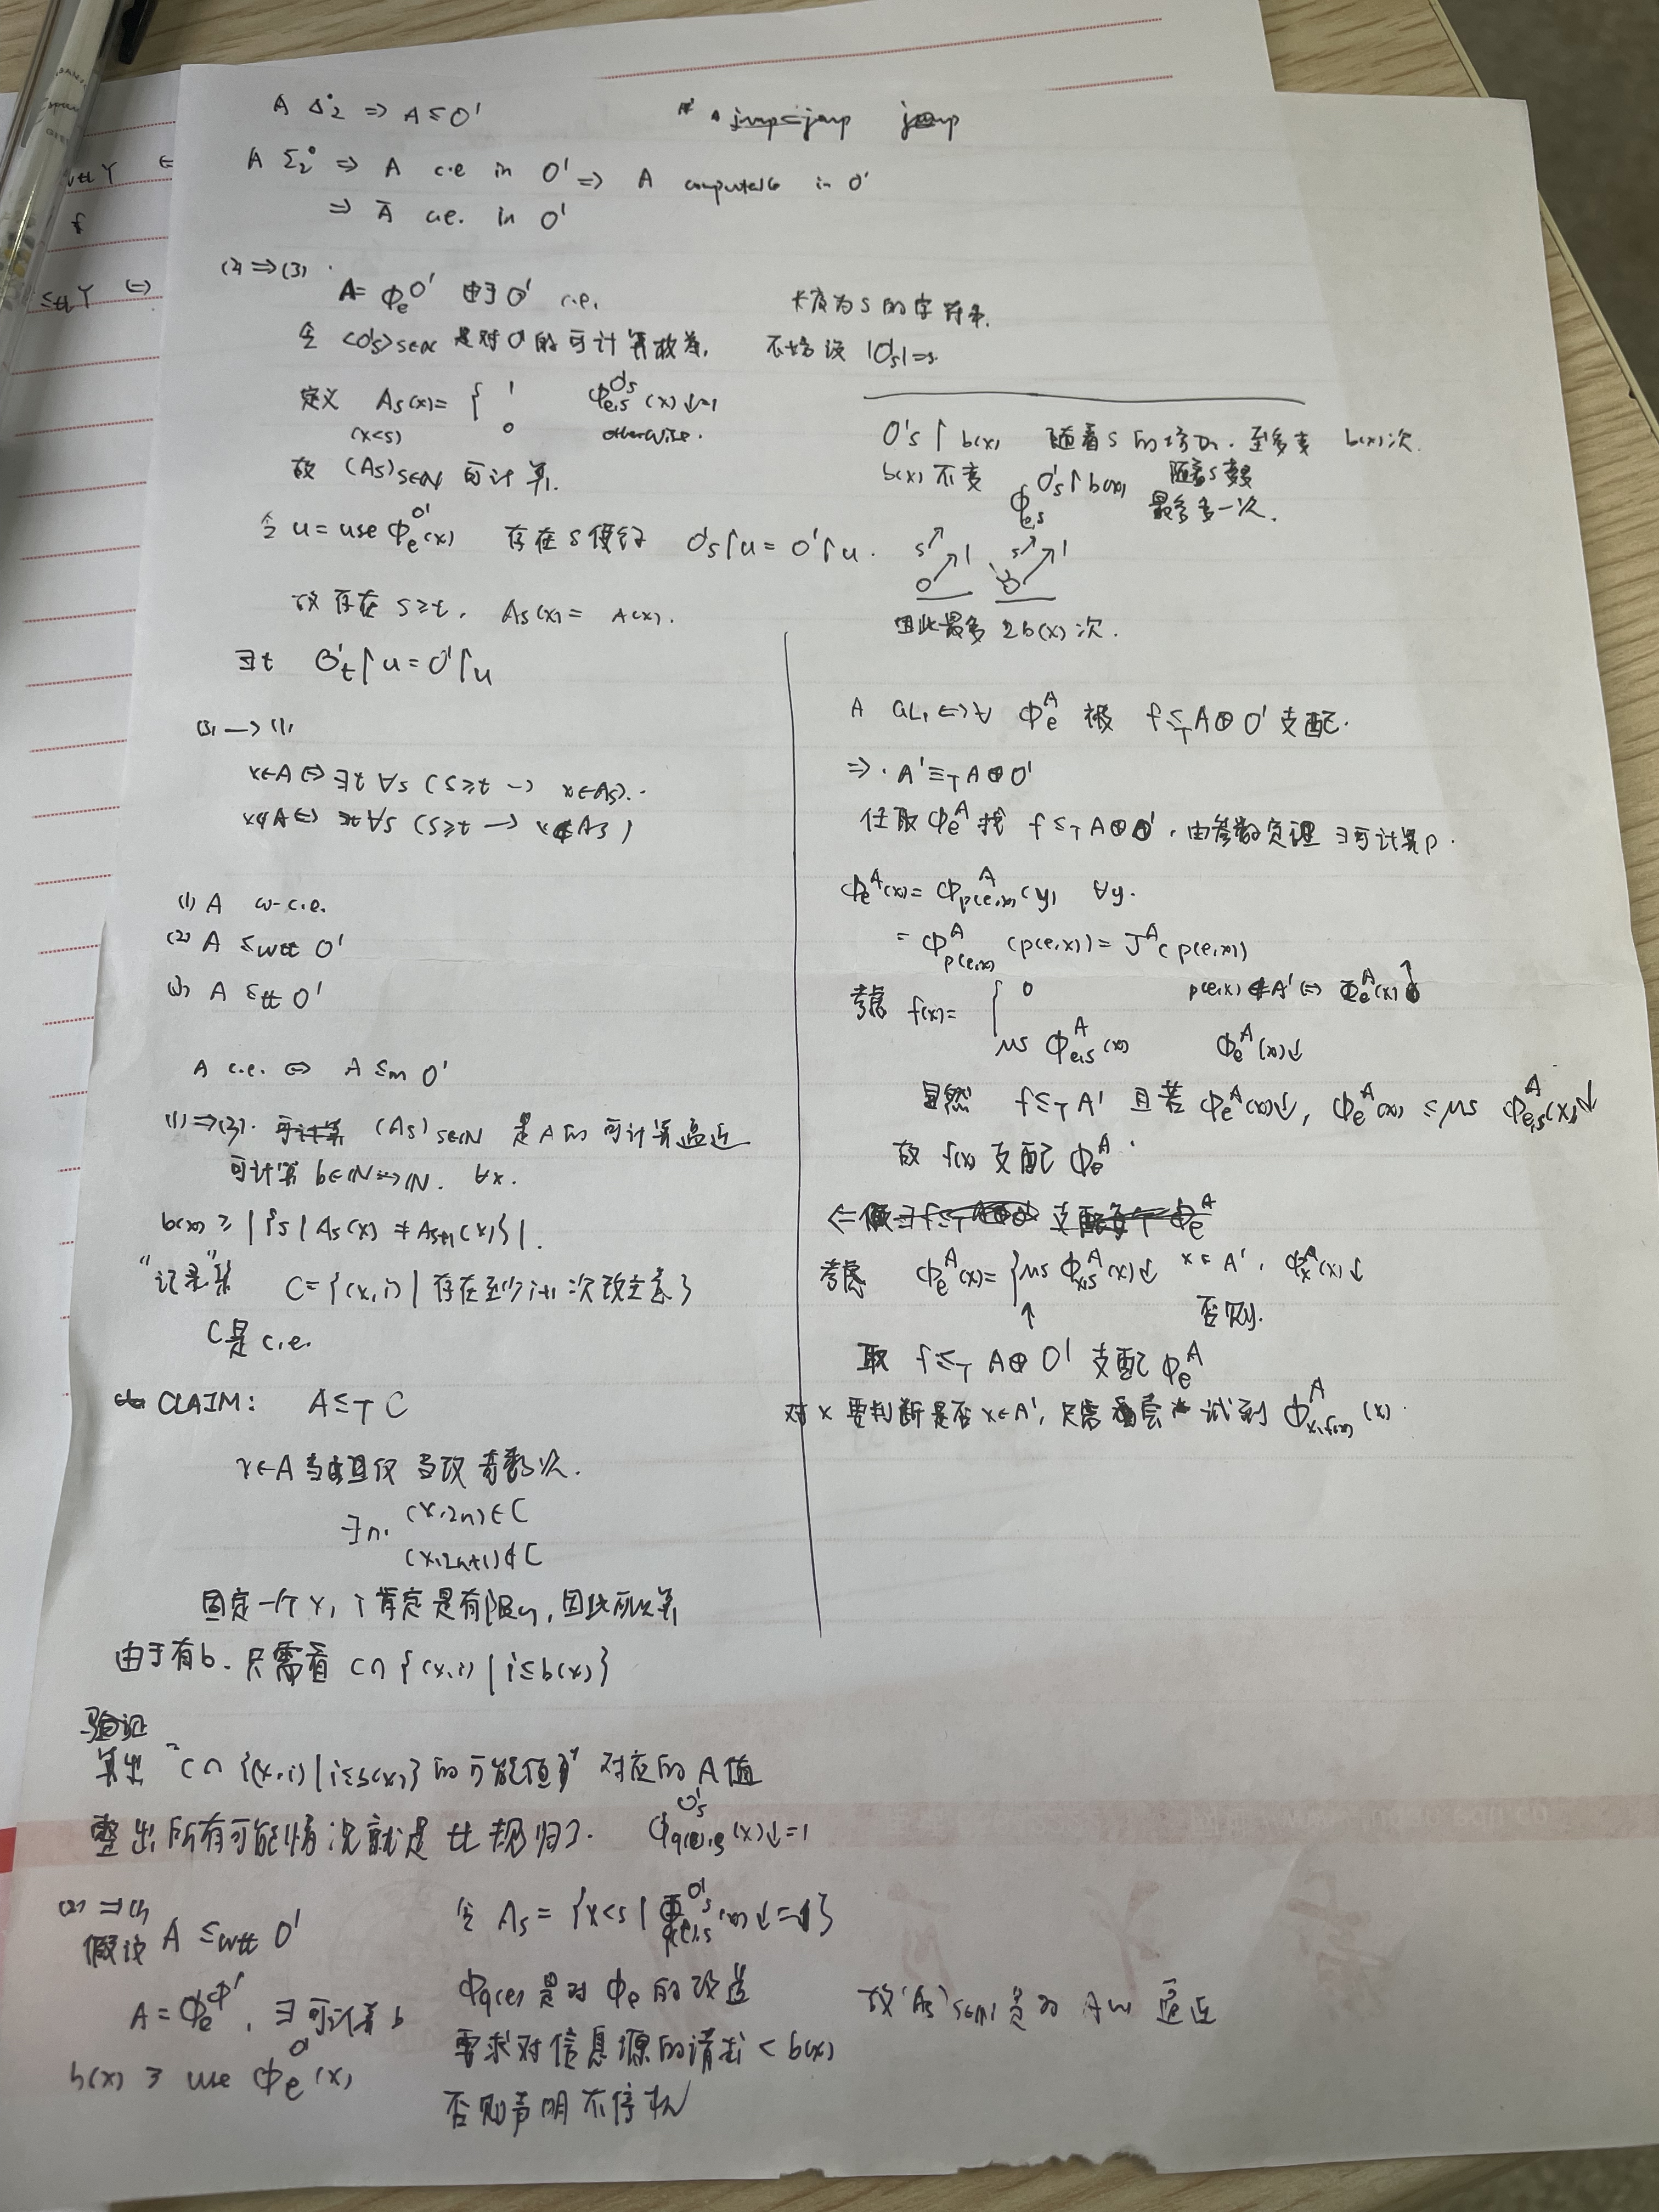
\includegraphics[width=.5\textwidth]{../images/clrs/1.png}
\label{}
\end{center}

The edge \((u,v)\) forms a cycle with the edges on the single path \(p\) from \(u\) to \(v\)
in \(T\). Since \(u\) and \(v\) are on opposite sides of the cut \((S,V-S)\), at least one edge
in \(T\) lies on the simple path \(p\)and also crosses the cut. Let \((x,y)\) be any such edge.
The edge \((x,y)\) is not in \(A\), because the cut respects \(A\).Since \((x,y)\) is on the
unique simple path from \(u\) to \(v\) in \(T\), removing \((x,y)\) breaks \(T\) into two
components. Adding \((u,v)\) reconnected them to form a new spanning
tree \(T'=(T-\{(x,y)\})\cup\{(u,v)\}\).

We next show that \(T'\) is a minimum spanning tree. Since \((u,v)\) is a light edge
crossing \((S,V-S)\) and \((x,y)\) also crosses this cut, \(w(u,v)\le w(x,y)\).
Therefore \(w(T')\le w(T)\).
\end{proof}

\begin{corollary}[]
Let \(G=(V,E)\) be a connected, undirected graph with a real-valued weight function \(w\)
defined on \(E\). Let \(A\) be a subset of \(E\) that is included in some minimum spanning tree
for \(G\), and let \(C=(V_C,E_C)\) be a connected component in the forest \(G_A=(V,A)\).
If \((u,v)\) is a light edge connecting \(C\) to some other component in \(G_A\), then \((u,v)\)
is safe for \(A\).
\end{corollary}
\subsubsection{The algorithms of Kruskal and Prim}
\label{sec:org7fbb10d}
\begin{enumerate}
\item Kruskal's algorithm
\label{sec:orgf4bc2e1}
Kruskal's algorithm finds a safe edge to add to the growing forest by finding, of all the edges
that connect any trees in the forest, an edge \((u,v)\) with the lowest weight.
\begin{algorithmic}[1]
\Procedure{MST-Kruskal}{$G,w$}
\State \(A=\emptyset\)
\For{each vertex \(v\in G.V\)}
    \State Make-Set\((v)\)
\EndFor
\State create a single list of the edges in \(G.E\)
\State sort the list of edges into monotonically increasing order by weight \(w\)
\For{each edge \((u,v)\) taken from the sorted list in order}
    \If{Find-Set(\(u\))\(\neq\)Find-Set(\(v\))}
        \State \(A=A\cup\{(u,v)\}\)
        \State Union(\(u,v\))
    \EndIf
\EndFor
\State \textbf{Return} \(A\)
\EndProcedure
\end{algorithmic}

The running time of Kruskal's algorithm for a graph \(G=(V,E)\) depends on the specific
implementation of the disjoint-set data structure.
\end{enumerate}

\subsection{Single-Source Shortest Paths}
\label{sec:org648f66e}
\begin{algorithmic}[1]
\Procedure{Initialize-single-source}{$G,s$}
\For{\(v\in G.V\)}
    \State \(v.d=\infty\)
    \State \(v.\pi=nil\)
\EndFor
\State \(s.d=0\)
\EndProcedure
\end{algorithmic}

\begin{algorithmic}[1]
\Procedure{Relax}{$u,v,w$}
\If{v.d\ge u.d+w(u,v)}
    \State \(v.d=u.d+w(u,v)\)
    \State \(v.\pi=u\)
\EndIf
\EndProcedure
\end{algorithmic}

\subsubsection{The Bellman-Ford algorithm}
\label{sec:org74e2030}
\begin{algorithmic}[1]
\Procedure{Initialize-single-source}{$G,s$}
    \For{\(i=1\) to \(\abs{G,V}-1\)}
        \For{\((u,v)\in G.E\)}
            \State RELAX\((u,v,w)\)
        \EndFor
    \EndFor
    \For{each edge \((u,v)=G.E\)}
        \If{\(v.d>u.d+w(u,v)\)}
            \State \textbf{return }False
        \EndIf
    \EndFor
\EndProcedure
\end{algorithmic}


\begin{lemma}[]
Let \(G=(V,E)\) be a weighted, directed graph with source \(s\) and weight function \(w:E\to\R\),
and assume that \(G\) contains no negative-weight cycles that are reachable from \(s\). Then
after the \(\abs{V}-1\) iterations of the \textbf{for} loops, we have \(v.d=\delta(s,v)\) for all
vertices \(v\) that are reachable from \(s\)
\end{lemma}

\begin{proof}
Consider any vertex \(v\) that is reachable from \(s\), and let \(p=\la v_0,v_1,\dots,v_k\ra\)
where \(v_0=s\) and \(v_k=v\) to be any shortest path from \(s\) to \(v\). Because shortest
paths are simple, \(p\) has at most \(\abs{V}-1\) edges, and so \(k\le\abs{V}-1\). Each of
the \(\abs{V}-1\) iterations of the \textbf{for} loop relaxes all \(\abs{E}\) edges. Among the edges
relaxed in the \(i\)th iteration, for \(i=1,\dots,k\), is \((v_{i-1},v_i)\). By the path-relaxation
property, therefore \(v.d=v_k.d=\delta(s,v_k)=\delta(s,v)\)
\end{proof}

\begin{corollary}[]
Let \(G=(V,E)\) be a weighted, directed graph with source vertex \(s\) and weight
function \(w:E\to\R\), and assume that \(G\) contains no negative-weight cycles that are reachable
from \(s\). Then for each vertex \(v\in V\) there is a path from \(s\) to \(v\) iff BELLMAN-FORD
terminates with \(v.d<\infty\) when it is run on \(G\)
\end{corollary}

\begin{theorem}[Correctness of the Bellman-Ford algorithm]
Let BELLMAN-FORD be run on a weighted, directed graph \(G=(V,E)\) with source \(s\) and weight
function \(w:E\to\R\). If \(G\) contains no negative-weight cycles that are reachable from \(s\),
then the algorithm return TRUE, we have \(v.d=\delta(s,v)\) for all vertices \(v\in V\), and the
predecessor subgraph \(G_\pi\) is a shortest-path tree rooted at \(s\). If \(G\) does contain a
negative-weight cycle reachable from \(s\), then the algorithm returns FALSE
\end{theorem}

\begin{proof}
Now suppose that graph \(G\) contains a negative-weight cycle that is reachable from the
source \(s\); let this cycle be \(c=\la v_0,\dots,v_k\ra\), where \(v_0=v_k\). Then
\begin{equation*}
\sum_{i=1}^kw(v_{i-1},v_i)<0
\end{equation*}
Assume for the purpose of contradiction that the Bellman-Ford algorithm returns TRUE.
Thus, \(v_i.d\le v_{i-1}.d+w(v_{i-1},v_i)\) for \(i=1,\dots,k\). Summing the inequalities around
cycle \(c\) gives us
\begin{align*}
\sum_{i=1}^kv_i.d&\le\sum_{i=1}^k(v_{i-1}.d+w(v_{i-1},v_i))\\
&=\sum_{i=1}^kv_{i-1}.d+\sum_{i=1}^kw(v_{i-1},v_i)
\end{align*}
But since \(\sum_{i=1}^kv_i.d=\sum_{i=1}^kv_{i-1}.d\), we have
\begin{equation*}
0\le\sum_{i=1}^kw(v_{i-1},v_i)
\end{equation*}
\end{proof}

\begin{exercise}

\end{exercise}
\subsubsection{Single-source shortest paths in directed acyclic graphs}
\label{sec:orgd5c692a}
By relaxing the edges of a weighted dag \(G=(V,E)\) according to a topological sort of its
vertices, we can compute shortest paths from a single source in \(\Theta(V+E)\) time. Shortest paths
are always well defined in a dag

\begin{algorithmic}[1]
\Procedure{Dag-Shortest-Paths}{$G,w,s$}
\State topological sort the vertices of \(G\)
\State INITIALIZE-SINGLE-SOURCE\((G,s)\)
\For{each vertex \(u\), taken in topological sorted order}
    \For{each vertex \(v\in G.Adj[u]\)}
        RELAX\((u,v,w)\)
    \EndFor
\EndFor
\EndProcedure
\end{algorithmic}

\begin{exercise}[24.2-4]
Given an efficient algorithm to count the total number of paths in a directed acylic graph.
Analyze your algorithm
\end{exercise}
\subsubsection{Dijkstra's algorithm}
\label{sec:orgb563df3}
Dijkstra's algorithm solves the single-source shortest-paths problem on a weighted, directed
graph \(G=(V,E)\) for the case in which all edge weights are nonnegative.
\begin{algorithmic}[1]
\Procedure{Dijkstra}{$G,w,s$}
\State \(S=\emptyset\)
\State \(Q=G.V\)
\While{\(Q\neq\emptyset\)}
    \State \(u=\)EXTRACT-MIN\((Q)\)
    \State \(S=S\cup\{u\}\)
    \For{each vertex \(v\in G.Adj[u]\)}
        RELAX\((u,v,w)\)
    \EndFor
\EndWhile
\EndProcedure
\end{algorithmic}

\begin{theorem}[Correctness of Dijkstra's algorithm]
Dijkstra's algorithm, run on a weighted, directed graph \(G=(V,E)\) with non-negative weight
function \(w\) and source \(s\), terminates with \(u.d=\delta(s,u)\) for all vertices \(u\in V\)
\end{theorem}

\begin{proof}
Let \(u\) be the first vertex for which \(u.d\neq\delta(s,u)\) when it is added to set \(S\).
Then \(u\neq s\) and \(\delta(s,u)\neq\infty\). Because there is at least one path, there is a shortest
path \(p\) from \(s\) to \(u\). Prior to adding \(u\) to \(S\), path \(p\) connects a vertex
in \(S\), namely \(s\) to a vertex in \(V-S\), namely \(u\). Let us consider the first
vertex \(y\) along \(p\) s.t. \(y\in V-S\), and let \(x\in S\) be \(y\)'s predecessor along \(p\).
We can decompose path \(p\) into \(s\xrsa{p_1}x\to y\xrsa{p_2}u\)

We claim that \(y.d=\delta(s,y)\) when \(u\) is added to \(S\). But \(y\) should be chosen after \(x\)
\end{proof}

\begin{exercise}

\end{exercise}
\subsubsection{Proofs of shortest-paths properties}
\label{sec:org292e937}
\begin{lemma}[Triangle inequality]
Let \(G=(V,E)\) be a weighted, directed graph with weight function \(w:E\to\R\) and source
vertex \(s\). Then for all edges \(u,v)\in E\) we have
\begin{equation*}
\delta(s,v)\le\delta(s,u)+w(u,v)
\end{equation*}
\end{lemma}

\begin{lemma}[Upper-bound property]
Let \(G=(V,E)\) be a weighted, directed graph with weight function \(w:E\to\R\). Let \(s\in V\) be
the source vertex, and let the graph be initialized by INITIALIZE-SINGLE-SOURCE\((G,s)\).
Then \(v.d\ge\delta(s,v)\) for all \(v\in V\), and this invariant is maintained over any sequence of
relaxation steps on the edges of \(G\). Moreover, once \(v.d\) achieves its lower
bound \(\delta(s,v)\) it never changes
\end{lemma}

\begin{proof}
By the inductive hypothesis, \(x.d\ge\delta(s,x)\) for all \(x\in V\) prior to the relaxation. The
only \(d\) that may change is \(v.d\). If it changes, we have
\begin{align*}
v.d&=u.d+w(u,v)\\
&\ge\delta(s,u)+w(u,v)\\
&\ge\delta(s,v)
\end{align*}
\end{proof}

\begin{corollary}[No-path property]
Suppose that in a weighted, directed graph \(G=(V,E)\) with weight function \(w:E\to\R\), no path
connects a source vertex \(s\in V\) to a given vertex \(v\in V\). Then, after the graph is
initialized by INITIALIZE-SINGLE-SOURCE\((G,s)\), we have \(v.d=\delta(s,v)=\infty\) and this equality is
maintained as an invariant over any sequence of relaxation steps on the edges of \(G\)
\end{corollary}

\begin{proof}
By the upper-bound property, we always have \(\infty=\delta(s,v)\le v.d\)
\end{proof}

\begin{lemma}[]
Let \(G=(V,E)\) be a weighted, directed graph with weight function \(w:E\to\R\), and
let \((u,v)\in E\). Then immediately after relaxing edge \((u,v)\) by executing RELAX\((u,v,w)\),
we have \(v.d\le u.d+w(u,v)\)
\end{lemma}

\begin{proof}
If prior to relaxing edge \((u,v)\), we have \(v.d>u.d+w(u,v)\), then \(v.d=u.d+w(u,v)\)
afterward. Otherwise \(v.d\) doesn't change
\end{proof}

\begin{lemma}[Convergence property]
Let \(G=(V,E)\) be a weighted, directed graph with weight function \(w:E\to\R\), let \(s\in V\) be a
source vertex, and let \(s\rightsquigarrow u\to v\) be a shortest path in \(G\) for some vertices \(u,v\in V\).
Suppose \(G\) is initialized by INITIALIZE-SINGLE-SOURCE\((G,s)\) and then a sequence of
relaxation steps that includes the call RELAX\((u,v,w)\) is executed on the edges of \(G\).
If \(u.d=\delta(s,u)\) at any time prior to the call, then \(v.d=\delta(s,v)\) at all times after the call
\end{lemma}

\begin{proof}

\end{proof}

\begin{lemma}[Path-relaxation property]
Let \(G=(V,E)\) be a weighted, directed graph with weight function \(w:E\to\R\), and let \(s\in V\)
be a source vertex. Consider any shortest path \(p=\la v_0,\dots,v_k\ra\) from \(s=v_0\) to \(v_k\).
If \(G\) is initialized by INITIALIZE-SINGLE-SOURCE\((G,s)\) and then a sequence of relaxation
steps occurs that includes, in order, relaxing the edges \((v_0,v_1),\dots,(v_{k-1},v_k)\)
then \(v_k.d=\delta(s,v_k)\) after these relaxations and at all times after wards.
\end{lemma}
\section{Dynamic Programming}
\label{sec:orgc46dd7c}
\subsection{Longest common subsequence}
\label{sec:orgbcb879e}
\begin{theorem}[Optimal substructure of an LCS]
Let \(X=\la x_1,\dots,x_m\ra\) and \(Y=\la y_1,\dots,y_n\ra\) be sequence, and let \(Z=\la z_1,\dots,z_k\ra\) be any LCS
of \(X\) and \(Y\).
\begin{enumerate}
\item If \(x_m=y_n\), then \(z_k=x_m=y_n\) and \(Z_{k-1}\) is an LCS of \(X_{m-1}\)
and \(Y_{n-1}\).
\item If \(x_m\neq y_n\) and \(z_k\neq x_m\), then \(Z\) is an LCS of \(X_{m-1}\) and \(Y\).
\item If \(x_m\neq y_n\) and \(z_k\neq y_n\), then \(Z\) is an LCS of \(X\) and \(Y_{n-1}\)
\end{enumerate}
\end{theorem}

\begin{proof}
\begin{enumerate}
\item If \(z_k\neq x_m\), then we could append \(x_m=y_n\) to \(Z\)
\end{enumerate}
\end{proof}
\end{document}